\documentclass{beamer}
\usetheme{default}
\beamertemplatenavigationsymbolsempty
\usepackage{rembeamer}

\begin{document}

\begin{frame}
  \begin{itemize}
    \item[] 
      Conducting hypothesis tests and constructing confidence
      intervals for a single proportion and interpreting the results.
  \end{itemize}
\end{frame}


\begin{frame}
  \frametitle{Single Proportions}
  \begin{itemize}
    \item[] 
      One categorical variable.
      \vspace{0.5cm}
    \item[] 
      Two categories. Interpreted as one success and one failure. 
      \vspace{0.5cm}
    \item[] 
      How many Canadians support the green party?
      \vspace{0.5cm}
    \item[] 
      How often do we have snow in September in Edmonton?
      \vspace{0.5cm}
    \item[] 
      How many restaurants in Edmonton have gluten-free options
      clearly available on their menus?
  \end{itemize}
\end{frame}

\begin{frame}
  \frametitle{An Example}
  \begin{itemize}
    \item[] 
      Survey of payday loan borrowers. 
      \vspace{0.5cm}
    \item[] 
      Question: do you support better regulation on payday loan
      lenders?
      \vspace{0.5cm}
    \item[] 
      826 Cases. Sample statistics: 70\% of these (578) answers
      ``yes''. 
      \vspace{0.5cm}
    \item[] 
      Question: is the population parameter greater than 65\%?
  \end{itemize}
\end{frame}

\begin{frame}
  \frametitle{Hypothesis Test}
  \begin{itemize}
    \item[] 
      Sample statistics: $\hat{p}= 0.70$
      \vspace{0.5cm}
    \item[] 
      Null hypothesis: $p = 0.65$
      \vspace{0.5cm}
    \item[] 
      Alternative hypothesis: $p > 0.65$
  \end{itemize}
\end{frame}

\begin{frame}
  \frametitle{Sampling Distribution}
  \centering
  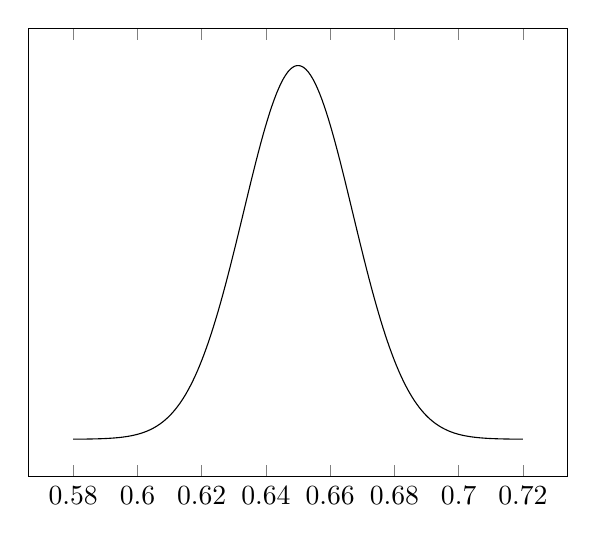
\begin{tikzpicture}
    \begin{axis}[
        ytick=\empty,
      ]
      \addplot [
        domain=0.58:0.72,
        samples=200,
      ]
      {exp(-(x-0.65)^2 / (2*(0.017)^2)) / (sqrt(2*pi*(0.017)^2))};
    \end{axis}
  \end{tikzpicture}
\end{frame}

\begin{frame}
  \frametitle{Sampling Distribution}
  \centering
  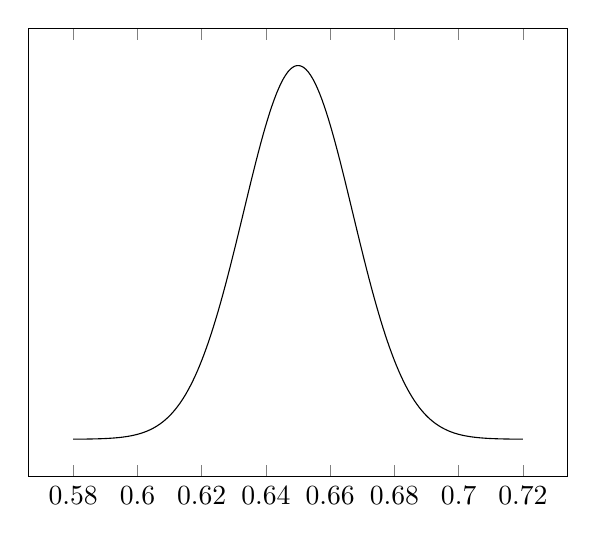
\begin{tikzpicture}
    \begin{axis}[
        ytick=\empty,
      ]
      \addplot [
        domain=0.58:0.72,
        samples=200,
      ]
      {exp(-(x-0.65)^2 / (2*(0.017)^2)) / (sqrt(2*pi*(0.017)^2))};
    \end{axis}
  \end{tikzpicture}
  \begin{equation*}
    \mu = 0.65 \hspace{2cm} \sigma = SE = ?
  \end{equation*}
\end{frame}

\begin{frame}
  \frametitle{Standard Error}
  \begin{displaymath}
    \begin{array}{rcl}
      SE & = & \sqrt{ \frac{p_1(1-p_1}{n_1} + \frac{p_2(1-p_2)}{n_2}
      }\\[2em]
      SE & = & \sqrt{ \frac{p(1-p)}{n}} 
    \end{array}
  \end{displaymath} 
\end{frame}

\begin{frame}
  \frametitle{Calculating p-value}
  \begin{displaymath}
    \begin{array}{rcl}
      x & = & 0.70 \\[2em]
      \mu & = & 0.65\\[2em]
      SE & = & \frac{(0.65)(1-0.65)}{826} = 0.017\\[2em]
      z(0.70) & = & 2.94 \\[2em]
      \text{percentile} & = & 0.998 \\[2em]
      p & = & 1 - 0.992 = 0.002 < 0.05 
    \end{array}
  \end{displaymath} 
\end{frame}

\begin{frame}
  \frametitle{Calculating Confidence Intervals}
  \begin{displaymath}
    \begin{array}{rcl}
      x & = & 0.70 \\[2em]
      \mu & = & 0.75\\[2em]
      SE & = & \frac{(0.75)(1-0.75)}{826} = 0.016\\[2em]
      \text{95\% Interval} &  = & [\mu - 1.96(SE), \mu + 1.96(SE)] \\[2em]
      \text{95\% Interval} &  = & [0.669,0.731] \\[2em]
    \end{array}
  \end{displaymath} 
\end{frame}

\end{document}
